\begin{abstractd}
Se resuelven dos modelos de ganancia de peso mediante ecuaciones diferenciales separables de primer orden. Para un becerro de 60 libras se obtiene la familia particular $w(t)=1200-1140e^{-kt}$, se representan los casos $k=0.8$, $0.9$ y $1$, y se calculan sus tiempos para alcanzar 800 libras. También se determina el peso límite de los tres modelos. Finalmente, para un peso inicial arbitrario $w_0$, se deduce la solución $w(t)=1200+(w_0-1200)e^{-t}$ y se comprueba por sustitución.
\end{abstractd}

\templateIndex

\section{Introducción}
Una ecuación diferencial relaciona una cantidad con su razón de cambio. En los problemas propuestos, la rapidez de ganancia de peso es proporcional a la diferencia entre el peso límite de $1200$ libras y el peso actual. Este comportamiento corresponde a un modelo de aproximación exponencial: la ganancia es rápida cuando el animal está lejos del límite y disminuye conforme se acerca a él \citep{stewart2016calculus,openstax2016calculus2}.

En todo el reporte, $w$ se mide en libras, $t$ en años y $k$ en años$^{-1}$. Se toma $t=0$ como el instante del nacimiento.

\section{Método de solución}
Para la ecuación
\[
 \frac{dw}{dt}=k(M-w),
\]
con $M=1200$, primero se observa que $w(t)=M$ es una solución constante. Para las soluciones no constantes, $M-w\neq0$ y se pueden separar las variables:
\begin{align*}
 \frac{dw}{M-w}&=k\,dt,\\
 \int\frac{dw}{M-w}&=\int k\,dt,\\
 -\ln|M-w|&=kt+C.
\end{align*}
Multiplicando por $-1$ y exponentiando:
\begin{align*}
 \ln|M-w|&=-kt-C,\\
 |M-w|&=e^{-C}e^{-kt}.
\end{align*}
El factor $e^{-C}$ es positivo; al retirar el valor absoluto, su signo se incorpora en una constante real $A$. Así,
\[
 M-w=Ae^{-kt},
 \qquad
 \boxed{w(t)=M-Ae^{-kt}}.
\]
El caso de equilibrio queda incluido al tomar $A=0$. La condición inicial permite determinar $A$, y la solución se verifica derivándola y sustituyéndola en la ecuación original.

\section{Problema 63: becerro de 60 libras}

\begin{examplebox}{Planteamiento y solución general}
Los datos son
\[
 w(0)=60,
 \qquad
 \frac{dw}{dt}=k(1200-w),
 \qquad k>0.
\]
La forma obtenida por separación es
\[
 w(t)=1200-Ae^{-kt}.
\]
Se aplica la condición inicial:
\begin{align*}
 60&=1200-Ae^0,\\
 60&=1200-A,\\
 A&=1200-60,\\
 A&=1140.
\end{align*}
Por tanto, el modelo para cualquier constante positiva $k$ es
\[
 \boxed{w(t)=1200-1140e^{-kt}}.
\]

\textbf{Comprobación:}
\[
 w'(t)=1140ke^{-kt}
 \quad\text{y}\quad
 k(1200-w)=k\bigl(1140e^{-kt}\bigr)=1140ke^{-kt}.
\]
Además, $w(0)=1200-1140=60$, de modo que se satisfacen tanto la ecuación diferencial como el dato inicial.
\end{examplebox}

\subsection{Inciso a: soluciones y representación gráfica}
Al sustituir los tres valores de $k$ se obtienen las soluciones:
\begin{align*}
 k=0.8:&\quad \boxed{w_{0.8}(t)=1200-1140e^{-0.8t}},\\
 k=0.9:&\quad \boxed{w_{0.9}(t)=1200-1140e^{-0.9t}},\\
 k=1.0:&\quad \boxed{w_{1.0}(t)=1200-1140e^{-t}}.
\end{align*}
Para atender la indicación de usar un sistema algebraico por computadora, se introdujeron la ecuación y la condición inicial en un solucionador simbólico. En notación de SymPy, la operación equivalente es
\[
 \operatorname{dsolve}\!\left(w'(t)=k(1200-w(t)),\;w(0)=60\right),
\]
cuyo resultado simplificado es $w(t)=1200-1140e^{-kt}$. Después se sustituyeron $k=0.8$, $0.9$ y $1$. La comprobación simbólica de cada resultado da
\[
 \operatorname{simplify}\!\left(w_k'(t)-k[1200-w_k(t)]\right)=0,
 \qquad w_k(0)=60.
\]

\begin{figure}[H]
\centering
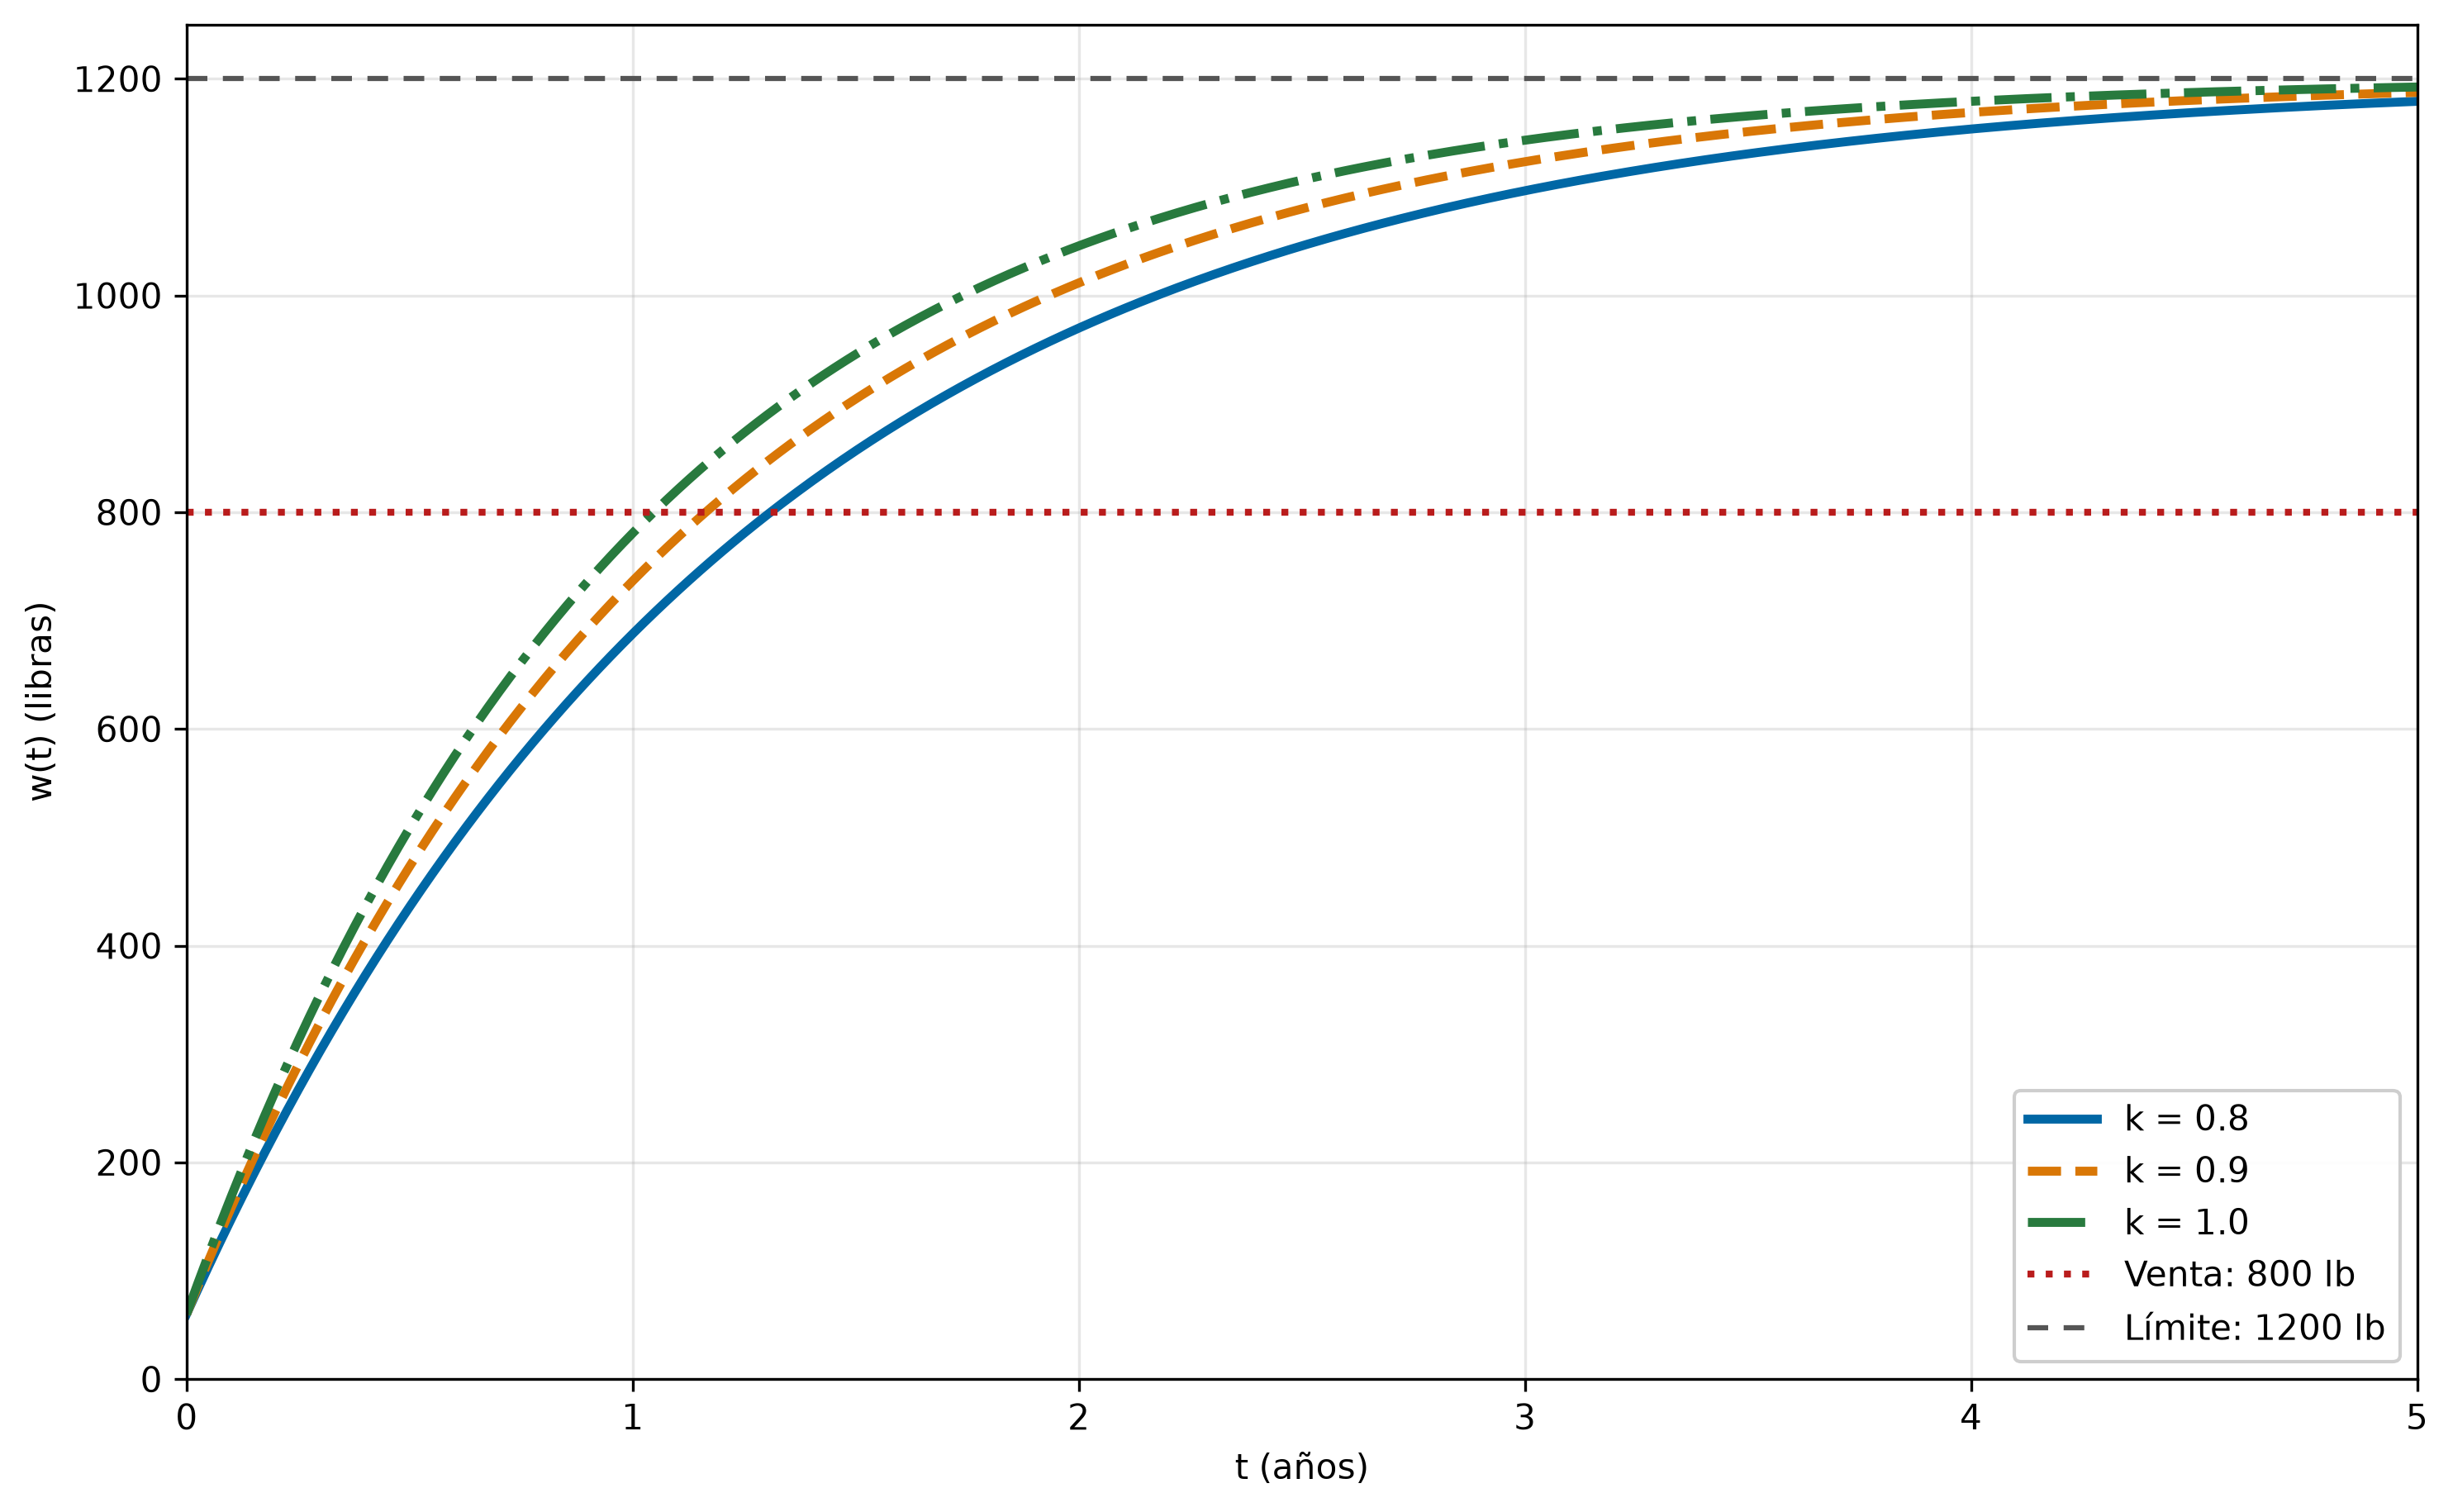
\includegraphics[width=0.94\textwidth]{UANL/ingeniero-agronomo/calculo-integral/assets-calculo-integral/modelos-ganancia-peso-actividad-2.png}
\caption{Soluciones del modelo de ganancia de peso para los tres valores de $k$.}
\label{fig:modelos-peso}
\end{figure}

La Figura~\ref{fig:modelos-peso} muestra que un valor mayor de $k$ produce una aproximación más rápida a 1200 libras. Las tres curvas parten de 60 libras y son crecientes, pero no rebasan el límite del modelo.

\subsection{Inciso b: tiempo de venta}
El animal se vende cuando $w(t)=800$. Para cualquier $k>0$:
\begin{align*}
 800&=1200-1140e^{-kt},\\
 1140e^{-kt}&=400,\\
 e^{-kt}&=\frac{400}{1140}=\frac{20}{57},\\
 -kt&=\ln\left(\frac{20}{57}\right),\\
 t&=-\frac{1}{k}\ln\left(\frac{20}{57}\right),\\
 \boxed{t_{\mathrm{venta}}=\frac{1}{k}\ln\left(\frac{57}{20}\right)}.
\end{align*}
La última igualdad usa $-\ln(a)=\ln(1/a)$. Como $\ln(57/20)\approx1.047319$, cada sustitución queda:
\begin{align*}
 t_{0.8}&=\frac{1.047319}{0.8}=1.309149\text{ años}
		  \approx 1.3091(12)=15.71\text{ meses},\\
 t_{0.9}&=\frac{1.047319}{0.9}=1.163688\text{ años}
		  \approx 1.1637(12)=13.96\text{ meses},\\
 t_{1.0}&=\frac{1.047319}{1}=1.047319\text{ años}
		  \approx 1.0473(12)=12.57\text{ meses}.
\end{align*}
Los resultados se resumen en la tabla siguiente:

\begin{table}[H]
\centering
\caption{Tiempo requerido para alcanzar 800 libras.}
\label{tab:tiempos-venta}
\begin{tabular}{ccc}
\toprule
$k$ (años$^{-1}$) & Tiempo exacto (años) & Tiempo aproximado \\
\midrule
$0.8$ & $\dfrac{1}{0.8}\ln\!\left(\dfrac{57}{20}\right)$ & $1.3091$ años ($15.71$ meses) \\
$0.9$ & $\dfrac{1}{0.9}\ln\!\left(\dfrac{57}{20}\right)$ & $1.1637$ años ($13.96$ meses) \\
$1.0$ & $\ln\!\left(\dfrac{57}{20}\right)$ & $1.0473$ años ($12.57$ meses) \\
\bottomrule
\end{tabular}
\end{table}

\textbf{Comprobación.} Si $t=(1/k)\ln(57/20)$, entonces
\begin{align*}
 e^{-kt}&=e^{-\ln(57/20)}=\frac{20}{57},\\
 w(t)&=1200-1140\left(\frac{20}{57}\right)
	=1200-400=800.
\end{align*}
Por tanto, los tres tiempos satisfacen exactamente la condición de venta. El modelo con $k=1$ llega primero al peso de venta y el de $k=0.8$ tarda más.

\subsection{Inciso c: peso máximo}
Para $t\geq0$ y $k>0$, el factor $e^{-kt}$ es positivo y tiende a cero cuando $t$ crece. Por ello,
\[
 w(t)=1200-1140e^{-kt}<1200
 \quad\text{para todo tiempo finito},
\]
y además
\[
 w'(t)=1140ke^{-kt}>0.
\]
Así, cada trayectoria es creciente y está acotada superiormente por 1200. Finalmente,
\[
 \lim_{t\to\infty}e^{-kt}=0
 \quad\Longrightarrow\quad
 \lim_{t\to\infty}\left(1200-1140e^{-kt}\right)=1200-1140(0),
\]
por lo que
\[
 \boxed{\lim_{t\to\infty}w(t)=1200\text{ libras}}.
\]
Así, los tres modelos tienen el mismo peso máximo límite de \textbf{1200 libras}. Con precisión matemática, 1200 libras es el supremo o valor asintótico: la función se aproxima indefinidamente, pero no lo alcanza en un tiempo finito. El parámetro $k$ modifica la rapidez de crecimiento, no el límite.

\section{Problema 64: peso inicial arbitrario}

\begin{examplebox}{Solución con $w(0)=w_0$}
Ahora se considera
\[
 \frac{dw}{dt}=1200-w,
 \qquad w(0)=w_0.
\]
Esta ecuación es el caso $k=1$ del modelo anterior. Si $w_0=1200$, se obtiene directamente la solución constante $w(t)=1200$. Para $w_0\neq1200$, se separan variables:
\begin{align*}
 \frac{dw}{1200-w}&=dt,\\
 \int\frac{dw}{1200-w}&=\int dt,\\
 -\ln|1200-w|&=t+C,\\
 \ln|1200-w|&=-t-C,\\
 |1200-w|&=e^{-C}e^{-t},\\
 1200-w&=Ae^{-t},\\
 w(t)&=1200-Ae^{-t}.
\end{align*}
Al retirar el valor absoluto, el signo se absorbe en la constante real $A$. La condición inicial determina esa constante:
\begin{align*}
 w_0&=1200-A,\\
 A&=1200-w_0.
\end{align*}
En consecuencia,
\begin{align*}
 \boxed{w(t)=1200-(1200-w_0)e^{-t}}
 &\qquad\text{o, equivalentemente,}\\
 \boxed{w(t)=1200+(w_0-1200)e^{-t}}.
\end{align*}
Esta fórmula también incluye el caso inicialmente separado $w_0=1200$, pues entonces el término exponencial es cero y $w(t)=1200$.

\textbf{Comprobación:}
\begin{align*}
 w'(t)&=-(w_0-1200)e^{-t}=(1200-w_0)e^{-t},\\
 1200-w(t)&=1200-\bigl[1200+(w_0-1200)e^{-t}\bigr]\\
 &=-(w_0-1200)e^{-t}=(1200-w_0)e^{-t}.
\end{align*}
Por tanto, $w'(t)=1200-w(t)$; además, $w(0)=1200+(w_0-1200)=w_0$.
\end{examplebox}

Si $0<w_0<1200$, el peso aumenta y se aproxima a 1200 libras. Si $w_0=1200$, la solución es constante. Aunque matemáticamente un valor $w_0>1200$ produciría una trayectoria decreciente hacia 1200, ese caso queda fuera de la interpretación habitual de ganancia de peso de un becerro recién nacido.

\section{Conclusiones}
La separación de variables permitió resolver ambos problemas y evidenciar el significado de sus parámetros. En el problema 63, las tres soluciones parten de 60 libras y comparten el límite de 1200 libras; aumentar $k$ únicamente reduce el tiempo necesario para acercarse a ese límite. Los tiempos de venta calculados son aproximadamente 1.3091, 1.1637 y 1.0473 años para $k=0.8$, $0.9$ y $1$, respectivamente. En el problema 64, el peso inicial queda incorporado en la constante de integración, dando una expresión válida para cualquier $w_0$. La derivación directa y la sustitución de las condiciones iniciales confirman todas las soluciones.

\begin{thebibliography}{4}
\bibitem[Hass et~al.(2018)]{thomas2018calculus}
Hass, J., Heil, C. y Weir, M. D. (2018).
\textit{Thomas' Calculus} (14.a ed.). Pearson.

\bibitem[Stewart(2016)]{stewart2016calculus}
Stewart, J. (2016).
\textit{Calculus: Early Transcendentals} (8.a ed.). Cengage Learning.

\bibitem[Strang y Herman(2016a)]{openstax2016calculus1}
Strang, G. y Herman, E. J. (2016a).
\textit{Calculus Volume 1}. OpenStax, Rice University.

\bibitem[Strang y Herman(2016b)]{openstax2016calculus2}
Strang, G. y Herman, E. J. (2016b).
\textit{Calculus Volume 2}. OpenStax, Rice University.
\end{thebibliography}
